\chapter{Conception}
  Ce chapitre présente l'architecture pensée pour la mise en \oe{}uvre d'un
  éditeur collaboratif utilisant \emph{Logoot} comme CRDT\footnote{Commutative
  Replicated Data Types}. La figure \ref{fig:architecture} représente cette
  architecture et sert de support aux explications qui suivent.

  \begin{figure}[h]
    \label{fig:architecture}
    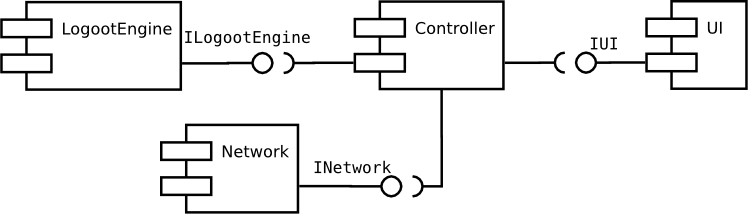
\includegraphics[width=\textwidth]{includes/architecture.png}
    \caption{Architecture d'un éditeur collaboratif utilisant \emph{Logoot}}
  \end{figure}

  Le \emph{LogootEngine} maintient le modèle de texte relatif à \emph{Logoot},
  c'est-à-dire la table des identifiants. Le \emph{LogootEngine} fournit un
  service de création d'un nouvel identifiant de ligne (lors de l'insertion
  d'un caractère à une position connue). Lorsque le système reçoit un
  patch\footnote{modèle de
  description des différences entre un document source et un document issue du
  document source} suite à des modifications sur le document effectuées par un
  autre utilisateur, \emph{Logoot} fournit un service permettant de l'intégrer
  au modèle déjà existant.

  Le composant \emph{Network} fournit des services d'envoi et de réception de
  données. Il est utilisé pour émettre un patch lors de modifications locales
  du document. De même, il est utilisé pour recevoir les patchs générés pas
  d'autres utilisateurs.

  L'\emph{UI}\footnote{User Interface} représente l'interface graphique de
  l'éditeur. Elle permet à l'utilisateur de visionner et modifier un document
  texte. L'\emph{UI} doit être notifiée de la mise à jour du document par un
  autre utilisateur, afin que l'utilisateur ait une vision toujours à jour
  du document partagé.

  Le \emph{Controller} sert à configurer le système. Il se charge de demander
  au \emph{LogootEngine} de mettre à jour sont modèle tout comme il notifie
  l'\emph{UI} des modifications des autres utilisateurs. C'est aussi lui qui se
  charge de transmettre les modifications locales sur le \emph{Network}. Il
  reçoit aussi, par le \emph{Network} les modifications des autres utilisateurs.

